%%%%%%%%%%%%%%%%%%%%%%%%%%%%%%%% Omslag %%%%%%%%%%%%%%%%%%%%%%%%%%%%%%%%

% CREATED BY DAVID FRISK, 2015

% COVER PAGE
\begin{titlepage}
\newgeometry{top=3cm, bottom=2.8cm,
			left=2.25 cm, right=2.25cm}	% Temporarily change margins		
			
% Cover page background 
\AddToShipoutPicture*{\backgroundpic{-4}{56.7}{frontpage_swe.pdf}}
\addtolength{\voffset}{2cm}

% Cover picture 
\begin{figure}[h!]
\centering
\vspace{2cm}	% Adjust vertical spacing here

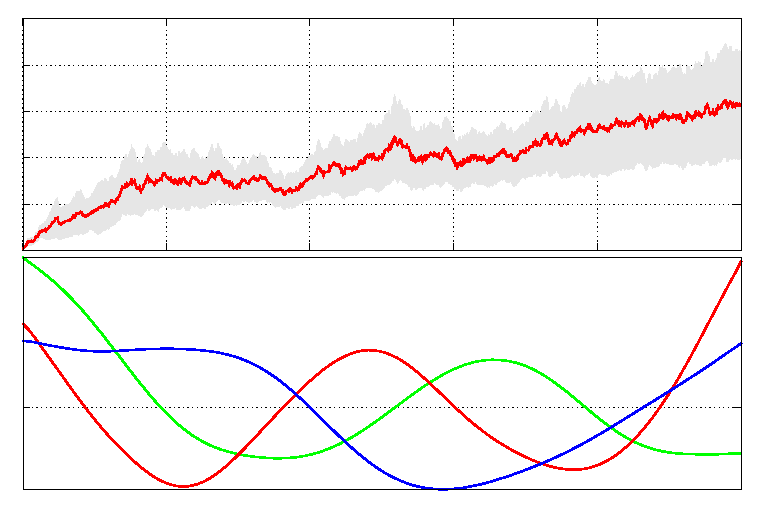
\includegraphics[width=0.9\linewidth,height=9cm]{cover.pdf}
\end{figure}

% Cover text
\mbox{}
\vfill
\renewcommand{\familydefault}{\sfdefault} \normalfont % Set cover page font

\begin{flushleft}
\textbf{{\Huge \titel }} 	\\[0.5cm]
{\Large \undertitel }       \setlength{\parskip}{0.5cm}

Kandidatarbete i Teknisk fysik \\[1cm]

{\Large 
ANDRÉAS SUNDSTRÖM \\%[0.5mm]
EMELIE EKENSTEDT \\%[0.5mm]
ROBIN KARLSSON \\%[0.5mm]
OLIVER SUNDELL\\[2cm]
} 
%1\vfill

\institution \\
\textsc{\skola} \\
Göteborg, Sverige 2016
\end{flushleft}

\renewcommand{\familydefault}{\rmdefault} \normalfont % Reset standard font
\end{titlepage}


% BACK OF COVER PAGE (BLANK PAGE)
\newpage
\restoregeometry
\thispagestyle{empty}
\mbox{}


%Bara en liten kodsnutt som behövs när man kompilerar lokalt
%%% Local Variables: 
%%% mode: latex
%%% TeX-master: "00main.tex"
%%% End: 